\documentclass{article}

\usepackage[tmargin=0.5in,bmargin=0.25in]{geometry}
\usepackage{amsmath, amssymb, amsthm}
\usepackage{listings}
\usepackage{multicol}
\usepackage{enumitem}
\usepackage{pgfplots}

\title{CSCI 305 Assignment 2}
\author{(Solo) Isaac Boaz}

\begin{document}
\maketitle

\begin{enumerate}
    \item  \begin{enumerate}[label=\arabic*.]
              \item Prove that finite sums and $\Theta$ commute.
                    \begin{equation*}
                        \sum_{i=1}^{n}{\Theta(f(i))} = \Theta(\sum_{i=1}^{n}{f(i)})
                    \end{equation*}
                    \begin{proof}
                        To show that finite sums and $\Theta$ commute, we must show that each has the same inequality constraints. \\[1em]
                        \textbf{Left-Hand Side}.
                        \begin{align*}
                                                                     & \sum_{i=1}^{n}{\Theta(f(i))}                              \\
                            \rightarrow \sum_{i=1}^{n}{c_1f(i)} \leq & \sum_{i=1}^{n}{\Theta(f(i))} \leq \sum_{i=1}^{n}{c_2f(i)} \\
                            \rightarrow c_1\sum_{i=1}^{n}{f(i)} \leq & \sum_{i=1}^{n}{\Theta(f(i))} \leq c_2\sum_{i=1}^{n}{f(i)}
                        \end{align*}
                        \textbf{Right-Hand Side}.
                        \begin{align*}
                                                                     & \Theta(\sum_{i=1}^{n}{f(i)})                              \\
                            \rightarrow c_1\sum_{i=1}^{n}{f(i)} \leq & \Theta(\sum_{i=1}^{n}{f(i)}) \leq c_2\sum_{i=1}^{n}{f(i)}
                        \end{align*}
                        Since both equations have the same lower and upper bounds, $\Theta$ is commutive.
                    \end{proof}
              \item Prove that \(\log_an = \Theta(\lg n)\) for any \(a > 1\), where \(\lg\) is \(\log_2\).
                    \begin{align*}
                        \log_an = \Theta(\lg n) \implies                          \\
                        \exists c_1, c_2, n_0 \in \mathbb{R}^+ \text{ such that } \\
                        c_1\lg n \leq \log_an \leq c_2\lg n \text{ for all } n \geq n_0
                    \end{align*}
                    Note that for any \(a\) or \(n\), we can set \(c_1 = 0\), Leaving us with the right-hand side of the equation.
                    \begin{align*}
                        \log_an                & \leq c_2 \lg n         \\
                        \frac{\log_2n}{log_2a} & \leq c_2 \log_2n       \\
                        c_2                    & \geq \frac{1}{\log_2a}
                    \end{align*}
                    Showing us that this holds true for any \(a > 1\).
                    \pagebreak
              \item Prove that for \(k\) integer, \(\sum_{i=1}^{n}{i^k} = \Theta(n^{k+1})\) \\
                    \begin{align*}
                        \sum_{i=1}^{n}{i^k} = \Theta(n^{k+1}) \implies \\
                        c_1n^{k+1} \leq \sum_{i=1}^{n}{i^k} \leq c_2n^{k+1}
                    \end{align*}
                    Similarly to the previous question, we can set \(c_1 = 0\) to resolve the lower bound.
                    As for the upper bound, notice
                    \begin{align*}
                        \sum_{i=1}^{n}{i^k} & \leq \sum_{i=1}^{n}{n^k} = n \cdot n^k = n^{k+1} \\
                        \sum_{i=1}^{n}{i^k} & \leq n^{k+1}
                    \end{align*}
                    hence \(\sum_{i=1}^{n}{i^k} = O(n^{k+1})\).
          \end{enumerate}
    \item  \begin{enumerate}[label=\arabic*.]
              \item Let \(p > 0\). Show that \(\log n = o(n^p)\). \\
                    To show that \(\log n = o(n^p)\), we must show that \(\lim_{n \to \infty}{\frac{\log n}{n^p}} = 0\).
                    \begin{align*}
                        \lim_{n \to \infty}{\frac{\log n}{n^p}} & = \lim_{n \to \infty}{\frac{\frac{1}{n}}{pn^{p-1}}} \\
                                                                & = \lim_{n \to \infty}{\frac{1}{pn^p}}               \\
                                                                & = 0
                    \end{align*}
              \item Let \(q > 0, p > 0\) Show that \(2^{qn} = \omega(n^p)\). \\
                    To show that \(2^{qn} = \omega(n^p)\), we must show that \(\lim_{n \to \infty}{\frac{2^{qn}}{n^p}} = \infty\).
                    \begin{align*}
                        \lim_{n \to \infty} \frac{2^{qn}}{n^p} & = \lim_{n \to \infty} \frac{qn2^{qn}}{pn^{p-1}} \\
                                                               & = \lim_{n \to \infty} \frac{qn2^{qn}}{pn^p}     \\
                                                               & = \lim_{n \to \infty} \frac{qn}{pn^p}           \\
                                                               & = \lim_{n \to \infty} \frac{q}{pn^{p-1}}        \\
                                                               & = \infty
                    \end{align*}
              \item \begin{figure}
                        \centering
                        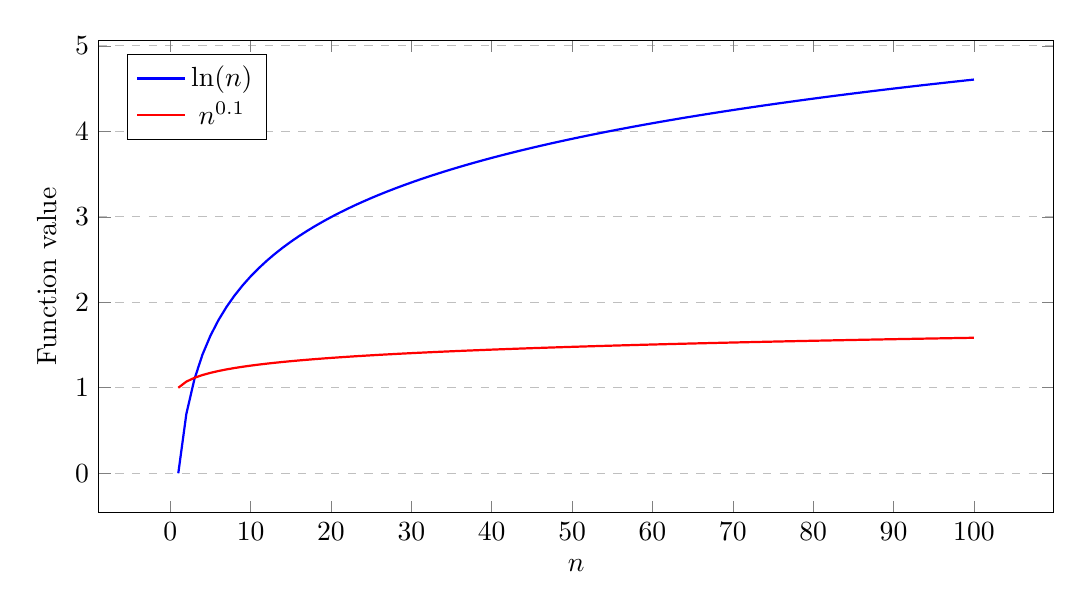
\begin{tikzpicture}
                            \begin{axis}[
                                    xlabel={$n$},
                                    ylabel={Function value},
                                    domain=1:100,
                                    legend pos=north west,
                                    ymajorgrids=true,
                                    grid style=dashed,
                                    scale only axis,
                                    width=\textwidth,
                                    height=6cm
                                ]

                                \addplot[blue, thick, samples=100] {ln(x)};
                                \addlegendentry{$\ln(n)$}

                                \addplot[red, thick, samples=100] {x^0.1};
                                \addlegendentry{$n^{0.1}$}
                            \end{axis}
                        \end{tikzpicture}
                        \caption{Plot of $\ln(n)$ and $n^{0.1}$}
                        \label{fig:inftyPlot}
                    \end{figure}
                    In Figure \ref{fig:inftyPlot} we see the plots of \(\ln(n)\) and \(n^{0.1}\). We can see that \(\ln(n)\) grows slower than \(n^{0.1}\) for all \(n > 1\). Note, however, that both functions have the same limit as \(n \to \infty\), namely \(\infty\).
          \end{enumerate}
          \pagebreak
    \item \begin{equation*}
              2^{\log x} \leq x \log x \leq x \log_{10} x \leq 2^x \leq e^{x \log x} \leq x!
          \end{equation*}
    \item Let \(F(1) = F(2) = 1\) be the `initial conditions' for the Fibonnaci recurrence given for \(n > 2\) by
          \begin{equation*}
              F(n) = F(n-1) + F(n-2)
          \end{equation*}
          \begin{enumerate}[label=\arabic*.]
              \item \begin{proof}
                        By induction. \\
                        \textbf{Base Case}: \(n = 1, n = 2\).
                        Observe at \(n = 1\), \(F(1) = 1\), and at \(n = 2\), \(F(2) = 1\) \\
                        Lastly, \(F(3) = F(2) + F(1) = 1 + 1 = 2 = \frac{a^3 - b^3}{\sqrt{5}}\). \\
                        \textbf{Inductive Step}: Assume \(F(n) = \frac{a^n - b^n}{\sqrt{5}}\) where \(a = \frac{1 + \sqrt{5}}{2}, b = \frac{1 - \sqrt{5}}{2}\). \\
                        Then (keeping in mind \(a^2 = a + 1\)) \begin{align*}
                            F(n+1) & = F(n) + F(n-1)                                                   \\
                                   & = \frac{a^n - b^n}{\sqrt{5}} + \frac{a^{n-1} - b^{n-1}}{\sqrt{5}} \\
                                   & = \frac{a^n - b^n + a^{n-1} - b^{n-1}}{\sqrt{5}}                  \\
                                   & = \frac{a^{n-1}(a + 1) - b^{n-1}(b + 1)}{\sqrt{5}}                \\
                                   & = \frac{a^{n-1}a^2 - b^{n-1}b^2}{\sqrt{5}}                        \\
                                   & = \frac{a^{n+1} - b^{n+1}}{\sqrt{5}}
                        \end{align*}
                    \end{proof}
              \item Using the formula from the previous question, we can show that \(F(n) = \Theta(a^n)\).
                    \begin{align*}
                        F(n) = \Theta(a^n) \implies                                    \\
                        \exists c_1, c_2, n_0 \in \mathbb{R}^+ \text{ such that }      \\
                        c_1x^n \leq F(n) \leq c_2x^n \text{ for all } n \geq n_0       \\
                        \rightarrow c_1x^n \leq \frac{a^n - b^n}{\sqrt{5}} \leq c_2x^n \\
                    \end{align*}
                    Note that for any \(n\) or \(x\), we can set \(c_1 = 0\) to resolve the lower bound, leaving us with the upper bound.
                    Since we know \(b\) is bounded by \(-1 \leq b \leq 0\), \(-1 \leq b^2 \leq 0\). Thus
                    \begin{align*}
                        \frac{a^n - b^n}{\sqrt{5}}                  & \leq \frac{a^n + 1}{\sqrt{5}}                               \\
                        \text{since the + 1 becomes proportionally} & \text{ smaller as } n \to \infty \text{, we can ignore it.} \\
                        \frac{a^n + 1}{\sqrt{5}}                    & \leq \frac{2a^n}{\sqrt{5}}                                  \\
                        \text{Leaving us with } c_2                 & = \frac{2}{\sqrt{5}} \text{ for any } n_0.
                    \end{align*}
          \end{enumerate}
    \item \phantom{a} \lstset
          { %Formatting for code in appendix
              language=Python,
              basicstyle=\footnotesize,
              numbers=left,
              stepnumber=1,
              showstringspaces=false,
              tabsize=1,
              breaklines=true,
              breakatwhitespace=false,
              numbersep=-30pt,
              xleftmargin=-20pt
          }
          \setlength{\columnseprule}{0.1pt}
          \begin{multicols}{2}
              \begin{lstlisting}
        for i = 1 to n
            for j = 1 to i
                k = 1
                    while k <= j
                        k = k +1
        \end{lstlisting}
              \columnbreak
              \footnotesize
              \begin{tabular}{l}
                  n + 1                                                   \\
                  $\sum_{i=1}^{n+1}{i}$                                   \\
                  $\sum_{i=1}^{n}{\sum_{j=1}^{i}{j}}$                     \\
                  $\sum_{i=1}^{n}{\sum_{j=1}^{i}{\sum_{k=1}^{j + 2}{k}}}$ \\
                  $\sum_{i=1}^{n}{\sum_{j=1}^{i}{\sum_{k=1}^{j + 1}{k}}}$
              \end{tabular}
          \end{multicols}
          The inner-most loop runs \(j + 1\) times, the middle loop runs \(i\) times, and the outer loop runs \(n\) times. Thus the total runtime is \(\Theta(n^3)\).
    \item [Ex. Credit] Prove
          \begin{equation*}
              \lim_{n \to \infty} \frac{f(n)}{g(n)} = C, \text{ } 0 \leq C \leq \infty \implies f(n) = \Theta(g(n))
          \end{equation*}
          First let's rewrite this using the definition of \(\Theta\).
          \begin{align*}
              \cdots \implies \exists c_1, c_2, n_0 \text{ such that } \\
              c_1g(n) \leq f(n) \leq c_2g(n) \text{ for all } n \geq n_0
          \end{align*}
          There are three cases to consider for \(C\). \\
          \textbf{Case 1}: \(C = 0\). \\
          This implies that \(g(n)\) grows much faster than \(f(n)\), meaning that \(f(n)\) is upper-bounded by \(g(n)\) for all \(n \geq n_0\). \\
          By this logic \(f(n) = O(g(n))\). \\[1em]
          \textbf{Case 2}: \(0 < C < \infty\). \\
          This implies that \(f(n)\) and \(g(n)\) grow at the same rate, meaning that \(f(n)\) is upper-bounded by \(g(n)\) and lower-bounded by \(g(n)\) for all \(n \geq n_0\). \\
          \begin{align*}
              C - \epsilon \leq \frac{f(n)}{g(n)}      & \leq C + \epsilon       \\
              \rightarrow (C - \epsilon)g(n) \leq f(n) & \leq (C + \epsilon)g(n)
          \end{align*}
          Thus \(f(n) = \Theta(g(n))\), where \(c_1 = C - \epsilon, c_2 = C + \epsilon\) \\[1em]
          \textbf{Case 3}: \(C = \infty\). \\
          This implies that \(g(n)\) grows much slower than \(f(n)\), meaning that \(f(n)\) is lower-bounded by \(g(n)\) for all \(n \geq n_0\). \\
          By this logic \(f(n) = \Omega(g(n))\). \\
\end{enumerate}


\end{document}